%%========================================================================
%% LaTeX scriptiesjabloon
%%========================================================================
%%========================================================================
%% Preamble
%%========================================================================

\documentclass[pdftex,a4paper,12pt,twoside]{report}

\usepackage{color}					 % kleur voor syntax highlighting
\usepackage{caption}
\usepackage{subcaption}
\usepackage[utf8]{inputenc}  % Accenten gebruiken in tekst (vb. � ipv \'e)
\usepackage{amsfonts}        % AMS math packages: extra wiskundige
\usepackage{amsmath}         %   symbolen (o.a. getallen-
\usepackage{amssymb}         %   verzamelingen N, R, Z, Q, etc.)
\usepackage[UKenglish]{babel}    % Taalinstellingen: woordsplitsingen,
                             %  commando's voor speciale karakters
                             %  ("dutch" voor NL)
                                                         %  ("UKenglish" voor brits engels)
\usepackage{eurosym}         % Euro-symbool �
\usepackage{graphicx}        % Invoegen van tekeningen
\usepackage[pdftex,bookmarks=true]{hyperref}
                             % PDF krijgt klikbare links & verwijzingen,
                             %  inhoudstafel
\usepackage{listings}        % Broncode mooi opmaken
\usepackage{multirow}        % Tekst over verschillende cellen in tabellen
\usepackage{rotating}        % Tabellen en figuren roteren
\usepackage{natbib}          % Betere bibliografiestijlen
\usepackage{fancyhdr}        % Pagina-opmaak met hoofd- en voettekst
\usepackage{footnote}
\usepackage{parskip}
\usepackage{longtable}			 % For tables longer than one page
\usepackage[final]{pdfpages}

% paragrafen zonder indentatie, en op andere lijn
\setlength{\parindent}{0pt }
\setlength{\parskip}{12pt plus 1pt minus 1pt}


\definecolor{dkgreen}{rgb}{0,0.6,0}
\definecolor{gray}{rgb}{0.5,0.5,0.5}
\definecolor{mauve}{rgb}{0.58,0,0.82}
\definecolor{darkgray}{rgb}{0.662745,0.662745,0.662745}
\definecolor{black}{rgb}{0,0,0}
\definecolor{lightgray}{rgb}{.9,.9,.9}
\definecolor{darkgray}{rgb}{.4,.4,.4}
\definecolor{purple}{rgb}{0.65, 0.12, 0.82}
\definecolor{darkblue}{rgb}{0.0,0.0,0.6}
\definecolor{cyan}{rgb}{0.0,0.6,0.6}


%%---------- Layout ------------------------------------------------------
\newcommand{\includecode}[2][c]{\lstinputlisting[caption=#2, escapechar=]{#2}}

% hoofdingen, enz.
\pagestyle{fancy}

% lijn, wordt gebruikt in titelpagina
\newcommand{\HRule}{\rule{\linewidth}{0.5mm}}

% Leeg blad
\newcommand{\emptypage}
{
	\newpage
	\thispagestyle{empty}
	\mbox{}
	\newpage
}
 
% Gebruik een schreefloos lettertype ipv het "oubollig" uitziende
% Computer Modern
\renewcommand{\familydefault}{\sfdefault}     

% Commando voor invoegen Java-broncodebestanden (dank aan Niels Corneille)
% Gebruik: \codefragment{source/MijnKlasse.java}{Uitleg bij de code}
\newcommand{\codefragmentjava}[2]
{ \lstset{%
  language=java,
  breaklines=true,
  float=th,
  caption={#2},
  basicstyle=\scriptsize,
  frame=single
}
\lstinputlisting{#1}}


\lstset{frame=tb,
  language=Java,
  aboveskip=3mm,
  belowskip=3mm,
  showstringspaces=false,
  columns=flexible,
  basicstyle={\small\ttfamily},
  numbers=left,
  numberstyle=\footnotesize,
  keywordstyle=\color{blue},
  commentstyle=\color{dkgreen},
  stringstyle=\color{mauve},
  breaklines=true,
  breakatwhitespace=true
  tabsize=3,
	captionpos=b,
	extendedchars=true
}

\lstdefinelanguage{JavaScript}
{
  keywords={typeof, new, true, false, catch, function, return, null, catch, switch, var, if, in, while, do, else, case, break},
  keywordstyle=\color{blue}\bfseries,
  ndkeywords={class, export, boolean, throw, implements, import, this},
  ndkeywordstyle=\color{darkgray}\bfseries,
  identifierstyle=\color{black},
  sensitive=false,
  comment=[l]{//},
  morecomment=[s]{/*}{*/},
  commentstyle=\color{purple}\ttfamily,
  stringstyle=\color{red}\ttfamily,
  morestring=[b]',
  morestring=[b]"
}

\lstdefinelanguage{XML}
{
  basicstyle=\ttfamily\color{darkblue}\bfseries,
  morestring=[b]",
  morestring=[s]{>}{<},
  morecomment=[s]{<?}{?>},
  stringstyle=\color{black},
  identifierstyle=\color{darkblue},
  keywordstyle=\color{cyan},
  morekeywords={xmlns,version,type}% list your attributes here
}


\lstdefinelanguage{CSS}
{
	alsodigit={-},
	ndkeywords={@import, @media, @page, @font-face, @charset, @namespace, @viewport, @-ms-viewport, @-o-viewport, @-moz-viewport, @-webkit-viewport, th},
  ndkeywordstyle=\color{darkgray}\bfseries,
  morekeywords={accelerator,azimuth,background,background-attachment,
    background-color,background-image,background-position,
    background-position-x,background-position-y,background-repeat,
    behavior,border,border-bottom,border-bottom-color,
    border-bottom-style,border-bottom-width,border-collapse,
    border-color,border-left,border-left-color,border-left-style,
    border-left-width,border-right,border-right-color,
    border-right-style,border-right-width,border-spacing,
    border-style,border-top,border-top-color,border-top-style,
    border-top-width,border-width,bottom,caption-side,clear,
    clip,color,content,counter-increment,counter-reset,cue,
    cue-after,cue-before,cursor,direction,display,elevation,
    empty-cells,filter,float,font,font-family,font-size,
    font-size-adjust,font-stretch,font-style,font-variant,
    font-weight,height,ime-mode,include-source,
    layer-background-color,layer-background-image,layout-flow,
    layout-grid,layout-grid-char,layout-grid-char-spacing,
    layout-grid-line,layout-grid-mode,layout-grid-type,left,
    letter-spacing,line-break,line-height,list-style,
    list-style-image,list-style-position,list-style-type,margin,
    margin-bottom,margin-left,margin-right,margin-top,
    marker-offset,marks,max-height,max-width,min-height,
    min-width,-moz-binding,-moz-border-radius,
    -moz-border-radius-topleft,-moz-border-radius-topright,
    -moz-border-radius-bottomright,-moz-border-radius-bottomleft,
    -moz-border-top-colors,-moz-border-right-colors,
    -moz-border-bottom-colors,-moz-border-left-colors,-moz-opacity,
    -moz-outline,-moz-outline-color,-moz-outline-style,
    -moz-outline-width,-moz-user-focus,-moz-user-input,
    -moz-user-modify,-moz-user-select,orphans,outline,
    outline-color,outline-style,outline-width,overflow,
    overflow-X,overflow-Y,padding,padding-bottom,padding-left,
    padding-right,padding-top,page,page-break-after,
    page-break-before,page-break-inside,pause,pause-after,
    pause-before,pitch,pitch-range,play-during,position,quotes,
    -replace,richness,right,ruby-align,ruby-overhang,
    ruby-position,-set-link-source,size,speak,speak-header,
    speak-numeral,speak-punctuation,speech-rate,stress,
    scrollbar-arrow-color,scrollbar-base-color,
    scrollbar-dark-shadow-color,scrollbar-face-color,
    scrollbar-highlight-color,scrollbar-shadow-color,
    scrollbar-3d-light-color,scrollbar-track-color,table-layout,
    text-align,text-align-last,text-decoration,text-indent,
    text-justify,text-overflow,text-shadow,text-transform,
    text-autospace,text-kashida-space,text-underline-position,top,
    unicode-bidi,-use-link-source,vertical-align,visibility,
    voice-family,volume,white-space,widows,width,word-break,
    word-spacing,word-wrap,writing-mode,z-index,zoom},
  morestring=[s]{:}{;},
	moredelim=[is][\color{black}\bfseries]{@*}{*@},
	moredelim=[is][\color{mauve}\bfseries]{@.}{.@},
	moredelim=[is][\color{blue}\bfseries]{@~}{~@},
	moredelim=[is][\color{red}\bfseries]{@�}{�@},
  sensitive,
  morecomment=[s]{/*}{*/}
}

%%---------- Documenteigenschappen ---------------------------------------
%% Vul dit aan met je eigen info:

% Je eigen naam
\newcommand{\studenta}{Kenzo Clauw}
\newcommand{\studentb}{Axl Fran\c{c}ois}
\newcommand{\studentc}{Lowie Huyghe}
\newcommand{\studentd}{Sander Trypsteen}
\newcommand{\studente}{Jelle Verreth}

% De titel van je scriptie/stageverslag
\newcommand{\titel}{Vakoverschrijdend Eindproject}

% Ondertitel
\newcommand{\ondertitel}{ Stambomen}

% Datum van indienen
\newcommand{\datum}{XX XXXX 2014}

% Academiejaar
\newcommand{\academiejaar}{2013-2014}

%%========================================================================
%% Inhoud document
%%========================================================================

\begin{document}

%%---------- Front matter ------------------------------------------------
%% Het voorblad - Hier moet je in principe niets wijzigen.

\begin{titlepage}
\begin{center}

\includegraphics[width=4cm]{images/logo.png}\\[.5cm]
Bachelor of Science Industrial Science : Informatics\\
Academic year \academiejaar

\vfill

\HRule \\[0.4cm]
{ \huge \bfseries \titel}\\[0.4cm]
\HRule \\[0.4cm]

{\Large \ondertitel}\\[0.4cm]

Submitted on \datum

\vfill

% Studenten en begeleiders
\begin{minipage}{0.49\textwidth}
\begin{flushleft}
\emph{Student\ifdefined\studentb s\fi :}\\
\studenta \\
\studentb \\
\studentc \\
\studentd \\
\studente
\par
\end{flushleft}
\end{minipage}
\begin{minipage}{0.49\textwidth}
\begin{flushright}
%\emph{Tutor:}\\ \begeleider\\
%\ifdefined\mentor \emph{Mentor:}\\ \mentor \fi
\end{flushright}
\end{minipage}

\end{center}

\end{titlepage}

% Schutblad

\emptypage

% Herhaling titelblad

\begin{titlepage}
\begin{center}
Master of Science Industrial Science : Informatics\\
Academic year \academiejaar

\vfill

\HRule \\[0.4cm]
{ \huge \bfseries \titel}\\[0.4cm]
\HRule \\[0.4cm]

{\Large \ondertitel}\\[0.4cm]

Submitted on \datum

\vfill

% Studenten en begeleiders
\begin{minipage}{0.49\textwidth}
\begin{flushleft}
\emph{Student\ifdefined\ \fi :}\\
\studenta \\
\studentb \\
\studentc \\
\studentd \\
\studente
%\ifdefined\studentb \studentb \fi\par
\end{flushleft}
\end{minipage}
\begin{minipage}{0.49\textwidth}
\begin{flushright}
%\emph{Tutor:}\\ \begeleider\\
%\ifdefined\mentor \emph{Mentor:}\\ \mentor \fi
\end{flushright}
\end{minipage}

\end{center}

\end{titlepage}

%% Inhoudstafel
\abstract


\tableofcontents

\chapter{Voorwoord}\label{ch:preface}

\paragraph{}
Dit projectdossier is een schriftelijk neerslag van onze prestaties voor het vakoverschrijvend project\footnote{VOP}. Hierin bespreken we de verschillende facetten van ons project. 
Allereest zullen wij beginnen met de opdracht voor te stellen en ze te situeren. Hierbij zullen we proberen van een zo volledig mogelijk overzicht te geven van alle technische en niet-technische onderdelen. Vervolgens krijgt u meer uitleg over de manier waarop onze takenverdeling tot stand komt en het volledig overzicht van onze takenverdeling.
Daarna bespreken we de analyse van het project aan de hand van enkele diagrammen en use cases. Vervolgens lichten we enkele belangerijke aspecten van ons project toe. We gaan hier zowel in op ontwerpbeslissingen als op implementatiekeuzes. Dan komen we aan de kwaliteitscontrole voldoet onze applicatie aan de fucntionele en niet-functionele veresiten zoals deze zijn opgesteld door de klant? Uiteraard zijn er in elk project wel problemen en we zullen het niet na laten om deze te bespreken. Als voorlaatste geven we nog even onze visie op het verdere verloop van de applicatie. Waar kan het beter, welke uitbreidingen zijn mogelijk. Ten slotte eindigen we met een nabeschouwing en ons besluit over het VOP.
\chapter{Introductie en situering}\label{ch:introduction}

\section{Introductie}
In deze paper kan u meer informatie vinden rond ons vop. Het onderwerp zoals u wellicht al gelezen hebt op het titel blad zijn stambomen. Het woord stambomen kan in verschillende contexten bekeken worden. We beperken ons echter enkel tot de genealogie. In genealogie zitten twee Griekse woorden verborgen namelijk Genea en Logos. Genea staat voor afkomst of afstamming en logos betekent wetenschap of kennis. 
Dus we bestuderen hier de afkomst, afstamming van een persoon.
In dit project zijn er echter twee bepererkingen:
\paragraph{}
Zonder dieper in te gaan op het onderwerp genealogie willen ook nog melden dat in dit project we ons slechts zullen beperken tot natuurlijk mogelijke afstammelingen. Hieronder verstaan wij dat er enkel man - vrouw relaties mogelijk zijn. We houden dus geen rekening met man - man of vrouw - vrouw relaties die dan kinderen zouden hebben.

\paragraph{}
Verder houden we ook geen rekening met de onderlinge relaties tussen echtparen. Op zich zijn dat onze zaken niet maar wanneer een persoon een buitenechtelijke kind heeft dan zal hij dat niet kunnen invoeren in ons programma. Hieronder vallen dus ook half-broers of half-zussen. Deze zullen niet weergegeven worden in ons stamboom overzicht.

\paragraph{}
Nu de scope van de opdracht duidelijker is kunnnen ingaan op wat er gevraagd is. Het is de bedoeling om een applicatie te maken waar een gebruiker stambomen kan ingeven en bekijken. De gebruiker moet deze stambomen kunnen raadplegen via een website  en de bomen worden ingegeven via een desktop applicatie. Verder moet de gebruiker ook zijn bomen kunnen delen met zijn vrienden zowel binnen de applicatie als op sociale netwerk sites. Voor dit project zullen we ons qua sociale netwerk sites beperken tot Facebook.

\section{Technische}
\paragraph{}
We hebben op 10/02/2014 de inleidende presentatie van het vop gekregen. Hierin werden een aantal vereisten uitgelegd. Deze vereisten staan uitgebreid beschreven in VOP: de richtlijnen \footnote{ADD REFERENCE}. De belangrijkste hierin zijn dat er een docent de rol van klant zal spelen. Er zullen afspraken moeten worden gemaakt met de klant over wat al dan niet mogelijk is. Wat er moet gerealiseerd worden? We kwamen ook te weten dat het project in Java moest geschreven worden. Verder moest dit gebeuren door aan de hand van een drielagen architectuur. 

\paragraph{Presentatie laag}
Deze laag bestond uit twee onderdelen namelijk een Java Desktop Client gemaakt in Java Swing en een website (HTML5, Javascript) die gebruikt maakt van Java Servlets. De nadruk uiteraard ligt hier bij het scheiden van onze logica van de presentatie.

\paragraph{Domein logica}
Hierbij was het de bedoeling om een REST-service in Java op te zetten waarvan de presentatie gebruik kan maken. We hebben hier van in het begin gekozen om Jersey te gebruiken.

\paragraph{Data tier}
Een relationele databank ging in staan voor de persistentie van onze gegevens. De databank die ons aangeboden werd door UGent is MySQL. We mochten in deze opdracht geen gebruik maken van ORM-tools\footnote{Object-Relational Mapping zoals Hibernate.}. 

\section{Situering}
\paragraph{}
WAT?

\chapter{Taak-verdeling}

\section{Methodologie}
\paragraph{}
Tijdens dit project zullen we gebruik maken van Scrum. Hierbij verdelen we het project in drie sprints. Aan het begin van elke sprint zitten we samen om te bespreken welke features we graag zouden opnemen. Hoe lang een bepaalde feature duurt om uit te werken. Na deze bespreking maken we een afspraak bij de klant.

\paragraph{}
Met de klant bespreken we dan welke features voor ons mogelijk zijn en welke features voor de klant noodzakelijk zijn. Hieruit volg een contract, alle features die we tijdens een bepaalde sprint zullen realiseren.

\paragraph{}
Op het einde van de sprint kijken we dan welke features we gerealiseerd hebben en welke niet. Dankzij deze methode kunnen we inschatten of we tijdens het project moeten bijsturen. Het kan zijn dat we niet alle features gerealiseerd hebben dan moeten we harder werken tijdens de volgende sprint.

\paragraph{}
Tijdens elke sprint krijgen we van de docenten een voorgestelde lijst met features.
Deze lijsten kan je vinden als appendix bij dit document,\ref{sec:opdrachtsprint1} en \ref{sec:opdrachtsprint2}
In het vervolg van dit hoofdstuk kan er dus wel eens verwezen worden naar de nummering die voor de taken gebruikt wordt in deze documenten.

\section{Sprint 1}

\subsection{Kenzo Clauw}

\begin{itemize}
\item 22. Het systeem bevat een grote hoeveelheid stamboomgegevens
\end{itemize}

\subsection{Axl François}

\begin{itemize}
\item Het aanmaken van de volledige structuur van de applicatie
\item 1. De gebruiker maakt een account aan.
\item 3. De gebruiker logt in op de desktopapplicatie.
\item 4. De gebruiker maakt een nieuwe stamboom aan.
\item 5. De gebruiker opent een bestaande stamboom.
\item 7. De gebruiker wijzigt de gegevens van een persoon in de huidige stamboom. 
\item 9. De gebruiker verwijdert een persoon uit de huidige stamboom (Niet afgewerkt)
\end{itemize}

\subsection{Lowie Huyghe}
\paragraph{WEB}
\begin{itemize}
\item 2. De gebruiker logt in op de webapplicatie.
\item 14. De gebruiker bekijkt zijn vriendenlijst.
\item 11. De gebruiker verstuurt een vriendschapsverzoek.
\item 12. De gebruiker aanvaardt een vriendschapsverzoek.
\item 13. De gebruiker weigert een vriendschapsverzoek.
\item 15. De gebruiker verwijdert iemand uit zijn vriendenlijst.
\item 16. De gebruiker consulteert zijn samengestelde stamboom.
\item 17. De gebruiker bekijkt de gegevens van een persoon in een stamboom.
\item 18. De gebruiker wijzigt de referentiepersoon van een stamboom.
\end{itemize}
\subsection{Sander Trypsteen}
\paragraph{API}
\begin{itemize}
\item 14. De gebruiker bekijkt zijn vriendenlijst.
\item 11. De gebruiker verstuurt een vriendschapsverzoek.
\item 12. De gebruiker aanvaardt een vriendschapsverzoek.
\item 13. De gebruiker weigert een vriendschapsverzoek.
\item 15. De gebruiker verwijdert iemand uit zijn vriendenlijst.
\end{itemize}
\subsection{Jelle Verreth}
\begin{itemize}
\item 4. De gebruiker maakt een nieuwe stamboom aan.
\item 6. De gebruiker voegt een persoon toe aan de huidige stamboom 
(Niet afgewerkt)
\item 8. De gebruiker verplaatst een persoon in de huidige stamboom 
(Niet afgewerkt)
\end{itemize}

\subsection{Niet opgenomen}
\begin{itemize}

\item 19. De gebruiker kiest de referentiepersoon voor de teletijdmachine. 
\item 20. De gebruiker kiest de datum voor de teletijdmachine
\item 21. De teletijdmachine markeert de geboorteplaatsen van de familieleden die op de ingevoerde 
datum in leven waren. 
\end{itemize}

\section{Sprint 2}

\subsection{Kenzo Clauw}
\begin{itemize}
\item 10. De gebruiker importeert een GEDCOM-bestand. 
\item 22. De moderator wijzigt de gegevens van een persoon. 
\item 23. De moderator wijzigt het profiel van een gebruiker. 
\item 24. De moderator blokkeert tijdelijk het account van een gebruiker. 
\end{itemize}

\subsection{Axl François}
\paragraph{Sprint 1}
\begin{itemize}
\item 6. De gebruiker voegt een persoon toe aan de huidige stamboom 
\item 8. De gebruiker verplaatst een persoon in de huidige stamboom 
\item 9. De gebruiker verwijdert een persoon uit de huidige stamboom
\end{itemize}
\paragraph{Desktop + API}
\begin{itemize}
\item 3. De gebruiker voegt een foto toe aan een persoon. 
\item 4. De gebruiker verwijdert een foto van een persoon.
\item 5. De gebruiker zoomt in op de stamboom. Naarmate meer ruimte beschikbaar is, worden meer 
gegevens weergegeven bij een persoon
\item 15. De gebruiker geeft aan of een stamboom wordt gedeeld met alle gebruikers van de applicatie, 
enkel met zijn/haar vrienden, of met niemand. 
\item 16. De gebruiker registreert zich met zijn/haar Facebookaccount. 
\item 17. De gebruiker koppelt zijn/haar account aan zijn/haar persoonlijke Facebookaccount. 
\item 18. De gebruiker logt in met Facebook. 
\item 30. De ontwikkelaar wijzigt de huisstijl van de applicatie.
\end{itemize}
 
\subsection{Lowie Huyghe}
\begin{itemize}
\item 7. De gebruiker doorzoekt de voor hem beschikbare stambomen
\item 25. De gebruiker bekijkt een animatie van de teletijdmachine. 
\item 26. De gebruiker vertraagt of versnelt de teletijdmachine. 
\item 27. De gebruiker pauzeert de teletijdmachine. 
\item 28. De gebruiker navigeert naar een tijdstip met de teletijdmachine
\item 29. De gebruiker wijzigt het thema van de applicatie.
\end{itemize}

\subsection{Sander Trypsteen}
\begin{itemize}
\item 12. De gebruiker doorzoekt de openbare gebruikerslijst. 
\item 13. De gebruiker bekijkt een openbaar profiel. 
\item 14. De gebruiker maakt zijn/haar profiel openbaar. 
\end{itemize}

\subsection{Jelle Verreth}
\begin{itemize}
\item 1. De gebruiker wijzigt deergavetaal. 
\item 2. Het systeem houdt een overzicht bij van relevante gebeurtenissen. 
\item 21. De gebruiker bekijkt een overzicht van de activiteiten van zijn/haar vrienden
\end{itemize}
\subsection{Niet opgenomen}
\begin{itemize}
\item 6. De gebruiker koppelt een persoon aan zijn/haar Facebookaccount. 
\item 8. De gebruiker geeft aan dat twee personen uit verschillende stambomen aan elkaar gelijk zijn. 
\item 9. Het systeem detecteert gelijkaardige personen uit verschillende stambomen en meldt de 
gelijkenissen aan de betrokken gebruikers. 
\item 10. De gebruiker bevestigt dat twee personen aan elkaar gelijk zijn. 
\item 11. De gebruiker geeft aan dat twee personen niet aan elkaar gelijk zijn.
\item 19. De gebruiker deelt stamboomgegevens op Facebook. 
\item 20. De gebruiker voegt een Facebookvriend toe aan zijn/haar vriendenlijst. 
\end{itemize}
  
\section{Sprint 3}

\subsection{Kenzo Clauw}
\begin{itemize}
\item 1. De gebruiker wijzigt de weergavetaal. 
\item 2. Het systeem houdt een overzicht bij van relevante gebeurtenissen. 
\end{itemize}
\subsection{Axl François}
\begin{itemize}
\item 6. De gebruiker koppelt een persoon aan zijn/haar Facebookaccount.
\end{itemize}
\subsection{Lowie Huyghe}
\begin{itemize}
\item 20. De gebruiker voegt een Facebookvriend toe aan zijn/haar vriendenlijst. 
\end{itemize}
\subsection{Sander Trypsteen}
\begin{itemize}
\item 19. De gebruiker deelt stamboomgegevens op Facebook. 
\item 18. De gebruiker logt in met Facebook.  (Web)
\end{itemize}
\subsection{Jelle Verreth}

\section{Overzicht}

\begin{tabular}{|c|c|c|c|c|c|}
\hline  & Kenzo Clauw & Axl Francois & Lowie Huyghe & Sander Trypsteen & Jelle Verreth \\ 
\hline SPRINT 1 &  &  &  &  &  \\
\hline 1. &  & \textcolor{red}{S1} &  &  &  \\ 
\hline 2. &  &  &  &  &  \\ 
\hline 3.  &  &  &  &  &  \\
\hline 4.  &  &  &  &  &  \\
\hline 5.  &  &  &  &  &  \\
\hline 6.  &  &  &  &  &  \\
\hline 7.  &  &  &  &  &  \\
\hline 8.  &  &  &  &  &  \\
\hline 9.  &  &  &  &  &  \\
\hline 10.  &  &  &  &  &  \\
\hline 11. &  &  &  &  &  \\ 
\hline 12. &  &  &  &  &  \\ 
\hline 13.  &  &  &  &  &  \\
\hline 14.  &  &  &  &  &  \\
\hline 15.  &  &  &  &  &  \\
\hline 16.  &  &  &  &  &  \\
\hline 17.  &  &  &  &  &  \\
\hline 18.  &  &  &  &  &  \\
\hline 19.  &  &  &  &  &  \\
\hline 20.  &  &  &  &  &  \\
\hline 21. &  &  &  &  &  \\ 
\hline 22. &  &  &  &  &  \\
\hline
\end{tabular}  
\newpage 
\begin{tabular}{|c|c|c|c|c|c|}
\hline  & Kenzo Clauw & Axl Francois & Lowie Huyghe & Sander Trypsteen & Jelle Verreth \\ 
\hline SPRINT 2 &  &  &  &  &  \\
\hline 1. &  & \textcolor{red}{S1} &  &  &  \\ 
\hline 2. &  &  &  &  &  \\ 
\hline 3.  &  &  &  &  &  \\
\hline 4.  &  &  &  &  &  \\
\hline 5.  &  &  &  &  &  \\
\hline 6.  &  &  &  &  &  \\
\hline 7.  &  &  &  &  &  \\
\hline 8.  &  &  &  &  &  \\
\hline 9.  &  &  &  &  &  \\
\hline 10.  &  &  &  &  &  \\
\hline 11. &  &  &  &  &  \\ 
\hline 12. &  &  &  &  &  \\ 
\hline 13.  &  &  &  &  &  \\
\hline 14.  &  &  &  &  &  \\
\hline 15.  &  &  &  &  &  \\
\hline 16.  &  &  &  &  &  \\
\hline 17.  &  &  &  &  &  \\
\hline 18.  &  &  &  &  &  \\
\hline 19.  &  &  &  &  &  \\
\hline 20.  &  &  &  &  &  \\
\hline 21. &  &  &  &  &  \\ 
\hline 22. &  &  &  &  &  \\
\hline 23.  &  &  &  &  &  \\
\hline 24.  &  &  &  &  &  \\
\hline 25.  &  &  &  &  &  \\
\hline 26.  &  &  &  &  &  \\
\hline 27.  &  &  &  &  &  \\
\hline 28.  &  &  &  &  &  \\
\hline 29.  &  &  &  &  &  \\
\hline 30.  &  &  &  &  &  \\
\hline 
\end{tabular} 

\paragraph{legende}
\begin{itemize}
\item Sprint 1: \textcolor{red}{S1}
\item Sprint 2: \textcolor{green}{S2}
\item Sprint 3: \textcolor{blue}{S3}
\item Sprint Niet opgenomen: \textcolor{cyan}{OP}
\item Sprint Niet afgewerkt: \textcolor{magenta}{AF}
\item Sprint Niet gerealiseerd: \textcolor{yellow}{GER}
\end{itemize}


\chapter{Analyse}

\chapter{Interresantee Ontwerpbeslissingen}

\chapter{Interessante Implementatiekeuzes}
\section{Bibliotheken}
\subsection{Jersey}

Jersey is een JAX-RS referentie-implementatie die een eigen API aanbied door de JAX-RS toolkit uit te breiden met extra functies en hulpprogramma's om op een eenvoudige manier RESTful Webservices en client development aan te bieden.
JAX-RS : Java API voor REST Web Services biedt ondersteuning bij het creëren van web services volgens het Representational State Transfer (REST) pattern.
REST is een pattern die beschrijft hoe resources geadresseerd en gebruikt kunnen worden.Een resource kan aangesproken worden dankzij een gemeenschappelijke interface op basis van de HTTP standaard methodes.
Een REST server zorgt ervoor dat de client een verbinding kan maken om de resources op te halen en te wijzigen. REST wordt veel gebruikt voor het bouwen van webservices en noemen we respectievelijk RESTful Webservices.
Voor de applicatie hebben we gebruik gemaakt van Jersey die zorgt voor de REST server en een REST client.


\subsection{Swagger Jersey}
Swagger is een specificatie en compleet uitvoeringskader voor het bescrijven, het produceren , consumeren en visualiseren van REST webservices. Het doel van Swagger om client en documentatie systemen de mogelijkheid te geven op hetzelfde tempo te werken als de server. De documentatie van de methoden,paremeters en modellen zijn nauw geïntegreerd in de server-code, waardoor de Apis altijd gesynchroniseerd zijn.

Door gebruik te maken van Swagger kunnen cliënten diensten consumeren en toegang tot de server code zonder in aanraking te komen de implementatie van de server.
De interface van het framework zorgt ervoor dat er interactie mogelijk is  met de API in een sandbox omgeving.
Swagger ondersteunt JSON en XML en zal in de toekomst ook beschikbaar zijn in andere formaten.






\subsection{SLF4J}
SLF4J is een Java logging api die gebruik maakt van een facade pattern, dit is een software design pattern die gebruikt wordt in object-oriented programming om een complex systeem voor te stellen als een interface.
De facade pattern is ideaal bij het werken met een groot aantal onderling afhankelijke klassen of klassen die meerdere methoden gebruiken , vooral wanneer deze te ingewikkeld zijn om te gebruiken of moeilijk te begrijpen.
De onderliggende logging backend van SLFJ4J wordt bepaald op runtime door het toevoegen van de gewenste binding aan het classpath ( java.util.logging).
Om gebruik te maken van SLF4J moet je de slf4j-api-1.7.7.jar en slf4j-simple-1.7.7.jar plaatsen in de classpath van het project.
Bij het volgende voorbeeld roepen we de loggerfactory op om dan vervolgens het toevoegen van een persoon te registeren :


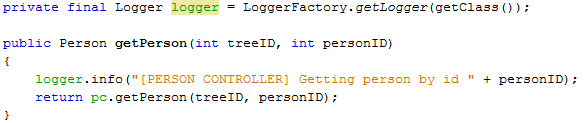
\includegraphics{images/logger.png}\\


\subsection{Junit 4.x}
JUnit is een unit testing framework voor Java die gebruikt wordt in test-driven development die deel uit maakt van xUnit.
Een unit test is een stukje code die een specifieke functionaliteit uitvoert om de code testen. Het percentage van de code die wordt getest door unit tests wordt meestal de test coverage genoemd.
Een unit test richt zich op een kleine eenheid van de code , bv een methode of een klasse.
Een integratie of functionele test eeft als doel om het gedrag van een component of de integratie tussen een set van componenten te testen.
Deze soort van testen kunnen user stories vertalen in een test suite , dit zou een soort sandbox omgeving zijn waarin alle methoden kunnen getest worden op bijvoorbeeld verkeerde input , lege waarden enz.
Naast integratie testen kan JUnit ook gebruikt worden voor het benchmarken van verschillende software componenten.

Aan de hand van een voorbeeld waarbij we een test unit maken voor de UserController is het eenvoudig om de verschillende mogelijkheden van JUnit uit te leggen.

Om in Netbeans een JUnit test aan te maken voor de UserController navigeer je naar het tools menu en klik je op Create Tests.

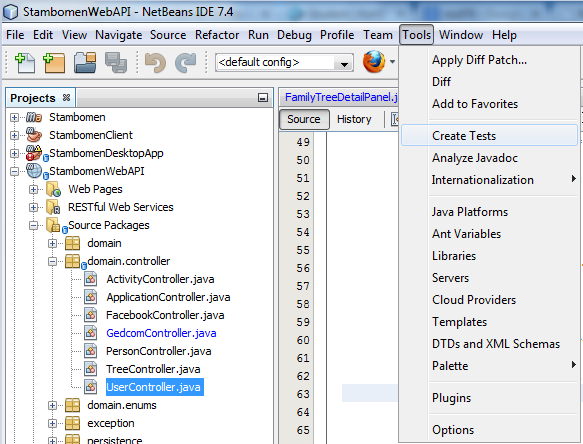
\includegraphics{images/netbeansjunit.png}\\

Er verschijnt een nieuw venster waarin er gevraagd wordt om een naam op te geven voor de JUnit test en welke code gegenereerd moet worden. Belangrijk hierbij is dat de class steeds moet eindigen op Test.

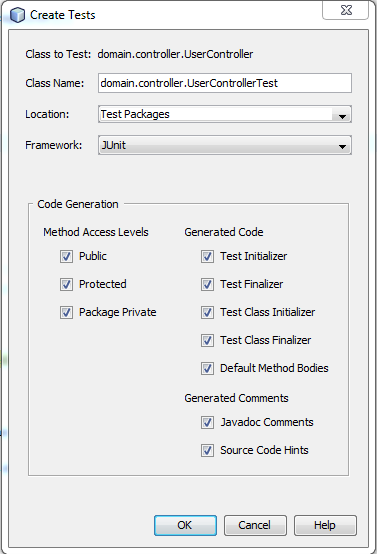
\includegraphics{images/netbeansjunit2.png}\\

Netbeans zal nu een nieuwe class aanmaken die een default constructor bevat die bij de UserControllerTest gebruikt wordt om de usercontroller , theme en user object aan te maken.

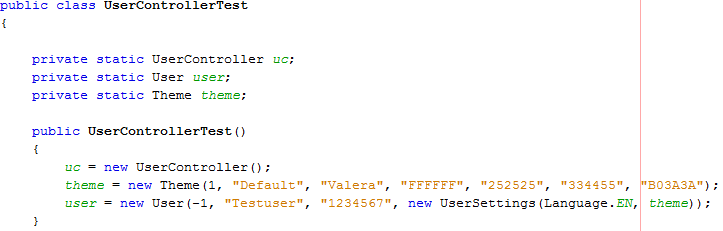
\includegraphics{images/junit1.png}\\

JUnit maakt gebruik van annotaties om de methoden die een test uitvoeren te identificeren en worden enkel opgenomen in een Test class. 
Een overzicht van de annotaties :

@Before and @After
Before en After zal worden aangeroepen voor en na elke test case.
Voor de UserControllerTest wordt dit gebruikt om de databank op te kuisen door de aangemaakte test gebruiker te verwijderen.

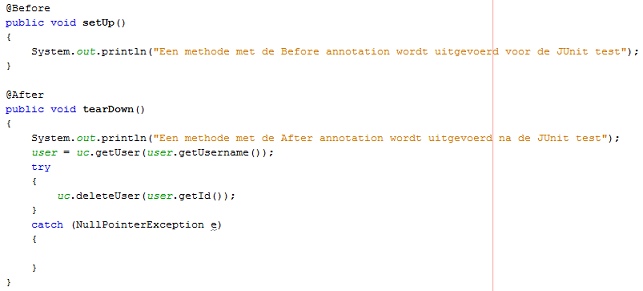
\includegraphics{images/beforeafter.png}\\


@BeforeClass and @AfterClass
Vergelijkbaar met Before and After maar deze zal pas worden utigevoerd na de JUnit Test en net voor of na de Class.

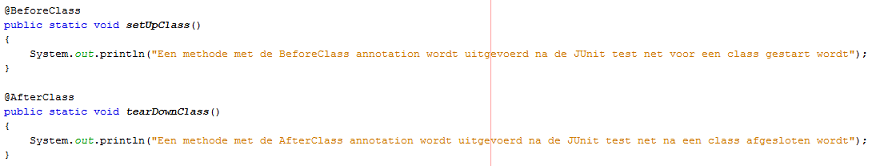
\includegraphics{images/beforeafterclass.png}\\

@Test
Een test annotatie wordt gebruik voor een normale test;

@Ignore
Wordt gebruikt om een bepaalde test over te slaan indien deze nog niet geïmplementeerd.
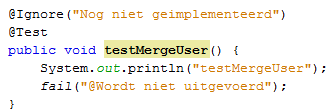
\includegraphics{images/junit2.png}\\

@Test(Timeout=500)
Het is mogelijk om een unit te testen na een bepaalde periode in milliseconden.

@Test (expected=IllegalArgumentException.class)
Soms is het nodig om te controleren of een bepaalde exceptie gesmeten wordt , in ons voorbeeld met de UsercontrollerTest is dit bij het opvangen van een gebruiker die al bestaat in de databank.

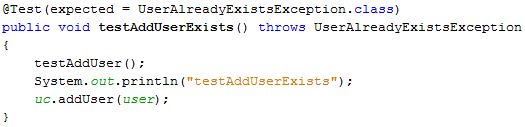
\includegraphics{images/junit3.png}\\

Assert statements

Junit biedst statische methoden aan in de Assert class die ervoor zorgen dat er testen kunnen opgesteld worden met bepaalde voorwaarden.
Een assert methode vergelijkt de werkelijke waarde die teruggegeven wordt door een test met de verwachte waarde en gooit een AssertException indien deze vergelijking mislukt.

Een overzicht van asserts:

fail(String)
een fail op het toevoegen van de user forceren.

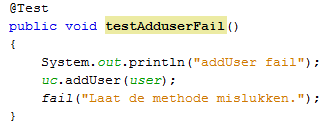
\includegraphics{images/adduserfail.png}\\

assertTrue(Bericht,boolean voorwaarde)
Controleert of de boolean voorwaarde waar is.

assertFalse(Bericht, boolean voorwaarde)
Controleert of de boolean voorwaarde onwaar is.

assertNull(bericht ,object)
Controleert of het object null is

assertNotNull(bericht ,object)
Controleert of het object niet null is.

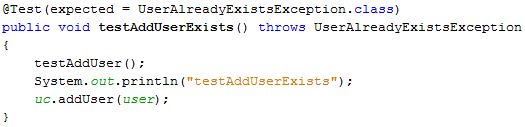
\includegraphics{images/junit3.png}\\

AssertEquals(bericht, verwacht ,werkelijk)
Test of twee waarden gelijk zijn.

Indien je met meerdere test klassen werkt kunt u deze combineren in een test suite.
Het uitvoeren van een testsuite bevat alle test classes van het project.




\subsection{Gedcom}

GEDCOM is een speciaal tekstformaat die ontwikkeld is door de Kerk van Jezus Christus van de Heiligen der Laatste Dagen en is bedoeld als standaard voor communicatie tussen de Kerk en personen die genealogische data aanleveren.
Dit formaat heeft zich nu ontwikkeld tot de standaard voor gegevensuitwisseling tussen de meeste genealogische programma's en systemen.

Stel dat we in de applicatie een persoon toevoegen dan zouden deze gegevens in een GEDCOM als volgt voorgesteld worden :

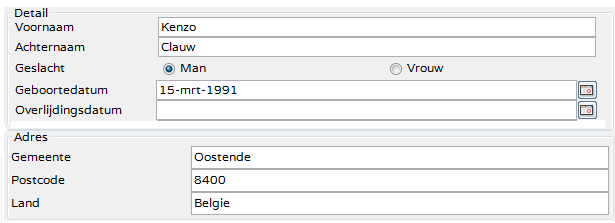
\includegraphics{images/gedcom.png}\\

Het eerste deel bevat de header met de gebruikte versie,character encoding (ANSEl,UNICODE of ASCII) als de belangrijkste informatie.


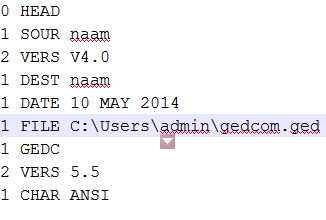
\includegraphics{images/gedcomheader.png}\\

Het tweede deel bevat informatie over de personen.

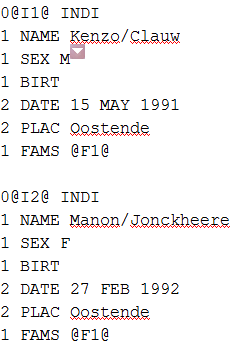
\includegraphics{images/gedcomperson.png}\\

Het laatste deel bevat de relaties tussen personen met TRLR die het bestand afsluit.

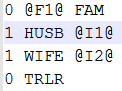
\includegraphics{images/gedcomrelaties.png}\\



\subsection{Gedcom4j}
Gedcom4j is een gratis open-source Java library voor het laden ( parsing ) en opslaan van gegevens in Gedcom genealogie 5.5 of 5.51 bestanden naar een Java-object hiërarchie.

Om gebruik te maken van Gedcom4j moet je de gedcom4j.jar plaatsen in de classpath van het project.

Om toegang tot gegevens te verkrijgen maak je gebruik van de properties binnen de gp.gedcom structure waarbij de personen voorgesteld worden door het object Individual en de relaties door Family.

Laden van een gedcom bestand :

GedcomParser gp = new GedcomParser();
gp.load("sample/TGC551.ged");

Om de personen te overlopen  :

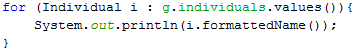
\includegraphics{images/gedcomindividual.png}\\

Om de relaties met kinderen te overlopen :

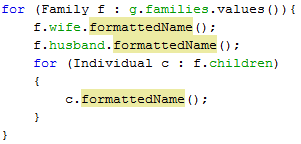
\includegraphics{images/gedcomfamily.png}\\

\subsection{Sardine}

Sardine is een WebDAV-client voor Java die een groot deel van de WebDAV client specificaties bevat. 

WebDAV is een uitbreiding op het HTTP protocol en staat voor Web-based Distributed Authoring and versioning.

Dit protocol wordt gebruik om op afstand bestanden aan te maken , wijzigen of te verplaatsen op een server via het internet.

De meeste moderne besturingssystemen ondersteunen WebDAV , waardoor een gebruiker bestanden op de server kan plaatsen alsof ze lokaal opgeslagen worden.

Gebruik :

Om gebruik te maken van Sardine plaats je de commons-logging.jar,commons-codec.jar en HttpClient/HttpCore 4.1.1 in je classpath.

Voor onze applicatie hebben we gebruik gemaakt van Sardine in de ImageDAO om images up te loaden naar de Server.


SardineFactory
Om gebruik te maken van Sardine interface maak je instantie van de SardineFactory aan om aan de hand van HTTP Authenticatie te verbinden met de WebDAV server.

\includegraphics{images/sardine.png}\\

Bij het doorgeven van credentials aan de client wordt de authenticatie scope geconfigureerd voor Basic , Digest en NTML verificatie om te reageren op de server.

put (String url, byte [] gegevens)
Aan de hand van HTTP put wordt een bestand op de server geplaats.

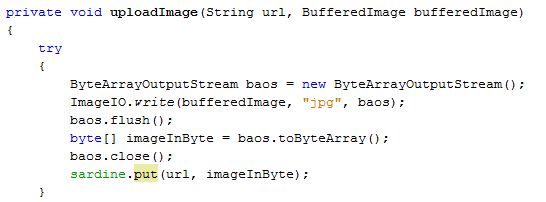
\includegraphics{images/sardineupload.png}\\



\subsection{RestFB}

RestFB is een efficiente Java implementatie van een Facebook Graph Api.
Het voordeel van RestFB is dat er ook ondersteuning is voor oudere versies van de API omdat sommige features nog niet geïmplementeerd zijn in de Graph API.

Registereren van een developer app :
Ga naar https://developers.facebook.com/apps om een nieuwe app te maken.

 
\includegraphics{images/facebook4.png}\\
 
 Een aanvraag bevestigen : 
 
 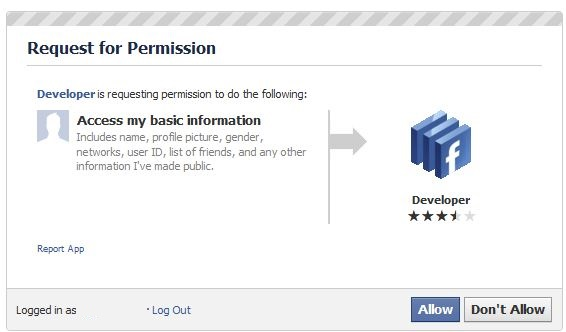
\includegraphics{images/facebook.png}\\
 
 Geef een naam op voor de nieuwe App Stambomen.
 
 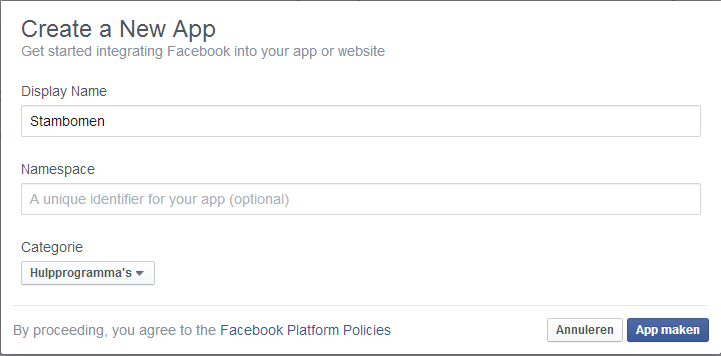
\includegraphics{images/facebook2.png}\\
 
 Op je dashboard verschijnt er een overzicht van je App met App-id en geheime code die gebruikt worden in de applicatie om een verbinding te maken.
 
 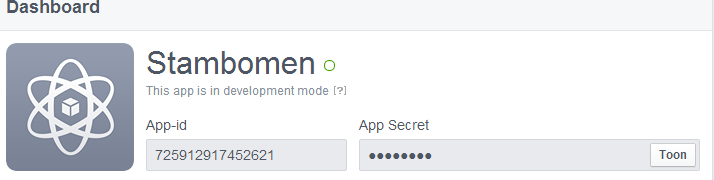
\includegraphics{images/facebook3.png}\\
 
Om in de applicatie in te loggen met facebook maak je een classFacebookClient aan waarin de secret code van de API vermeld wordt.

\includegraphics{images/facebook4.png}\\

Om een user op te vragen roep je in de FacebookClient de methode fetchObject op.

 

\subsection{JCalendar}
JCalender is een Java-date chooser om grafisch een datum te selecteren en bestaat uit een combinatie van de volgende componenten :

JDateChooser

Om een datum te kiezen kan je ofwel de datum rechtstreeks invullen of klikken op de afbeelding om de datum te kiezen.
De default date editor vangt de nodige fouten op met een respectievelijke rode kleur.


JDayChooser

Om een dag te kiezen klik je op het dag nummer die hoort bij de weeknummers en dagen die afhankelijk zijn van de locale.



JMonthChooser

Een JCombobox  waarbij een maand kan geselecteerd worden uit een keuzelijst of door de knoppen te verhogen / verlagen. De taal waarin de namen worden vermeld zijn afhankelijk van de Locale.
 
JYearChooser

Een JSpinField die het toelaat om een jaar te selecteren door de knoppen te verhogen / verlagen of deze manueel in het tekstveld invoeren.




\subsection{Abego TreeLayout}
ABEGO TreeLayout is een Efficiënt en aanpasbare Boom Layout algoritme voor Java.
De TreeLayout creëert boom lay-outs voor willekeurige bomen. Het is niet beperkt tot een bepaalde productie of formaat, maar kan worden gebruikt voor elke vorm van tweedimensionale tekening. Voorbeelden zijn Swing gebaseerde componenten, SVG-bestanden, en nog veel meer.

Om de Treelayout te gebruiken moet je een instantie van de klasse TreeLayout voorzien van de knooppunten van de boom inclusief zijn kinderen samen met de hoogte tussen verchillende niveaus.

Eigenschappen :
Op basis van deze informatie zorgt de TreeLayout voor een compacte layout met een overzichtelijke boom.

De indeling toont de hiërarchische structuur van de boom, namelijk de y-coördinaat van een knooppunt wordt bepaald door het niveau.

De randen kruisen elkaar niet en de nodes op hetzelfde niveau hebben een minimale horizontale afstand.
De volgorde van de kinderen van een knooppunt wordt weergegeven in de tekening.

Het algoritme werkt symmetrisch, dat wil zeggen de tekening van de weerspiegeling van een boom is het gereflecteerde tekening van de oorspronkelijke boom


Om gebruik te maken van de Abego TreeLayout moet je de org.abego.treelayout.core.jar(de TreeLayout algoritme kern) en org.abego.treelayout.netbeans.jar( gebruikt  van de NetBeans visuele API ) plaatsen in de classpath van het project.


\subsection{Java FX}
JavaFX is een platform die gebruikt wordt om Rich Internet Applications te ontwikkelen die audio,video en webservices aanbieden en kan gebruikt worden op computers of smartphones.
Rich Internet Applications zijn interactieve internetapplicaties die het gevoel van een desktopprogramma geven.

Omdat JavaFX gebaseerd is op Java is het platformonafhankelijk met als voordeel dat alle Java-bibliotheken kunnen worden gebruikt bij het ontwikkelen van applicaties.
Applicaties worden geschreven in JavaFX Script , een decleratieve scripttaal die speciaal is ontwikkeld voor webontwikkelaars en designers die visuaal willen programmeren. 
De applicaties in JavaFX kunnen worden uitgevoerd in een webbrowsers of kunnen worden geïnstalleerd  door ze naar het bureaublad  te slepen;
 
 \chapter{Kwaliteitscontrole}
 

Om de kwaliteit van onze applicatie te garanderen wordt er gebruik gemaakt van Test-driven development die een onderdeel is van agile softwareontwikkeling.

Hoe werkt Test-driven development?

Voor dat er code geschreven wordt maak je eerst een geautomatiseerde test waarbij je rekening moet houden met alle mogelijkheden van invoer , errors en uitvoer. Op deze manier moet je nog geen rekening houden met code.
De eerste keer dat een test uitgevoerd wordt moet deze een error produceren omdat er nog geen code aanwezig is.
Na het afwerken van de test is het de bedoeling om op basis van de tests code te schrijven.
Eens de code met succes de verschillende testen kan doorstaan kun je bepaalde bugs uit je applicatie al uitsluiten.

Voor onze applicatie hebben we gekozen voor JUNIT die het mogelijk maakt om aan de hand van functionele of integratie testen te debuggen volgens de opgestelde use cases.


Wat moet er getest worden?

In het algemeen is het veilig om bepaalde methoden zoals getters en setters die gewoon waarden oproepen of toewijzen te negeren. Het schrijven van tests hiervoor is tijdrovend en zinloos omdat je op deze manier de Java Virtual Machine zou testen waarvoor er al testen voorzien zijn.

Het is aangeraden om voor de kritische en complexe onderdelen van uw een applicatie uitgebreide testen te voorzien. Een stevige test suite beschermt u ook tegen regressie in de bestaande code als je nieuwe features introduceert.




\chapter{Gekende problemen}

\chapter{Verbeterpunten en uitbreidingsmogelijkheden}

Er zijn nog verschillende uitbreidingsmogelijkheden voor de applicatie die kunnen onderverdeeld worden volgens :
\subsection{Gedcom}
\begin{enumerate}
\item \label{it:first} Exporteren van gedcom bestanden
	Op de documentatie pagina van Gedcom4j staat er een perfect voorbeeld van hoe een GEDCOM bestand kan opgesteld worden met de nodige controle door een gedcomvalidator vanaf nul.
	http://gedcom4j.org/main/example-creating-gedcom-scratch
\item \label{it:first}  Meerdere stambomen uit een gedcom bestand importeren
	Bij het importeren van een gedcom bestand in de huidige applicatie is het enkel mogelijk om een stamboom te importeren waarvan alle relaties aan elkaar geknoopt zijn.
	Een uitbreiding zou ervoor kunnen zorgen dat meerdere stambomen opgesteld worden uit eenzelfde bestand.
\item \label{it:first} Toevoegen van een gedcom bestand aan een stamboom
\end{enumerate}

 
\subsection{Stambomen}
\begin{enumerate}
\item \label{it:first} Printen van een stamboom
\item \label{it:first} Personen verplaatsen tussen stambomen
\item \label{it:first} Samenvoegen van stambomen
\item \label{it:first} In 3D wandelen door een stamboom
\item \label{it:first} Exporteren en importeren van stambomen in bepaalde formaten zoals pdf , word , excel ,scv ..
\end{enumerate}

\subsection{Admin}

In de huidige applicatie bestaat het admin gedeelte enkel uit een Useroverviewpanel die een overzicht bevat van alle gebruikers.
Deze gebruikers kunnen door de admin geblokkeerd of gewijzigd worden en is er een mogelijkheid om in te loggen als een geselecteerde gebruiker om de gegevens van hun stamboom te wijzigen.
Het inloggen als een gebruiker door de admin heeft als voordeel dat de administrator een duidelijk beeld krijgt van zijn stambomen waarbij er niet te veel gegevens uit de databank opgehaald moeten worden.
Een uitbreidingsmogelijkheid zou zijn om een personoverviewpanel te voorzien om direct gegevens te wijzigingen in een lijst van personen.
Tijdens sprint 2 is er een prototype ontwikkelt die een lijst bevat van alle personen maar qua performantie was dit ver van ideaal.
Om het personoverviewpanel te verbeteren zouden de personen moeten verspreid worden door eerst een lijst te voorzien van de gebruikers , gevolgd door hun stambomen en dan pas een lijst van personen die aan de hand van paginering opgehaald worden uit de databank. 

Naast het personoverviewpanel zou de administrator de mogelijkhed moeten krijgen om volgende opties uit te voeren :
\begin{enumerate}
\item \label{it:first} Het importeren van gegevens uit andere databanken die gebruik maken van de applicatie
\item \label{it:first} Een statistisch overzicht van de verschillende acties in de applicatie
\end{enumerate}









Naast uitbreidingsmogelijkheden zijn er ook nog enkele verbeteringspunten :

\begin{enumerate}
\item \label{it:first} Bij het wijzigen van de user in de useroverviewpanel worden alle users terug opgehaald na een wijziging , het zou efficienter zijn om enkel de gewijzigde persoon terug op te halen.
\end{enumerate}



\chapter{Nabeschouwing en besluit}


%%%%%%%%%%%%%%%%%%%%%%%%%%%%%%%%%%%%%%%%%%%%%%%%%%%%%%%%%%%%%
%% BIBLIOGRAPHY AND OTHER LISTS
%%%%%%%%%%%%%%%%%%%%%%%%%%%%%%%%%%%%%%%%%%%%%%%%%%%%%%%%%%%%%
%% A small distance to the other stuff in the table of contents (toc)
\addtocontents{toc}{\protect\vspace*{\baselineskip}}

%% The Bibliography
%% ==> You need a file 'literature.bib' for this.
%% ==> You need to run BibTeX for this (Project | Properties... | Uses BibTeX)
%\addcontentsline{toc}{chapter}{Bibliography} %'Bibliography' into toc
%\nocite{*} %Even non-cited BibTeX-Entries will be shown.
%\bibliographystyle{alpha} %Style of Bibliography: plain / apalike / amsalpha / ...
%\bibliography{literature} %You need a file 'literature.bib' for this.

%% The List of Figures
\clearpage
\addcontentsline{toc}{chapter}{List of Figures}
\listoffigures

%% The List of Tables
\clearpage
\addcontentsline{toc}{chapter}{List of Tables}
\listoftables

%%%%%%%%%%%%%%%%%%%%%%%%%%%%%%%%%%%%%%%%%%%%%%%%%%%%%%%%%%%%%
%% APPENDICES
%%%%%%%%%%%%%%%%%%%%%%%%%%%%%%%%%%%%%%%%%%%%%%%%%%%%%%%%%%%%%

\appendix
\chapter{Appendix}


\includepdf[pages=-,pagecommand=\section{Opdracht sprint 1}\label{sec:opdrachtsprint1}, scale=0.80]{Files/stambomen-sprint1.pdf}
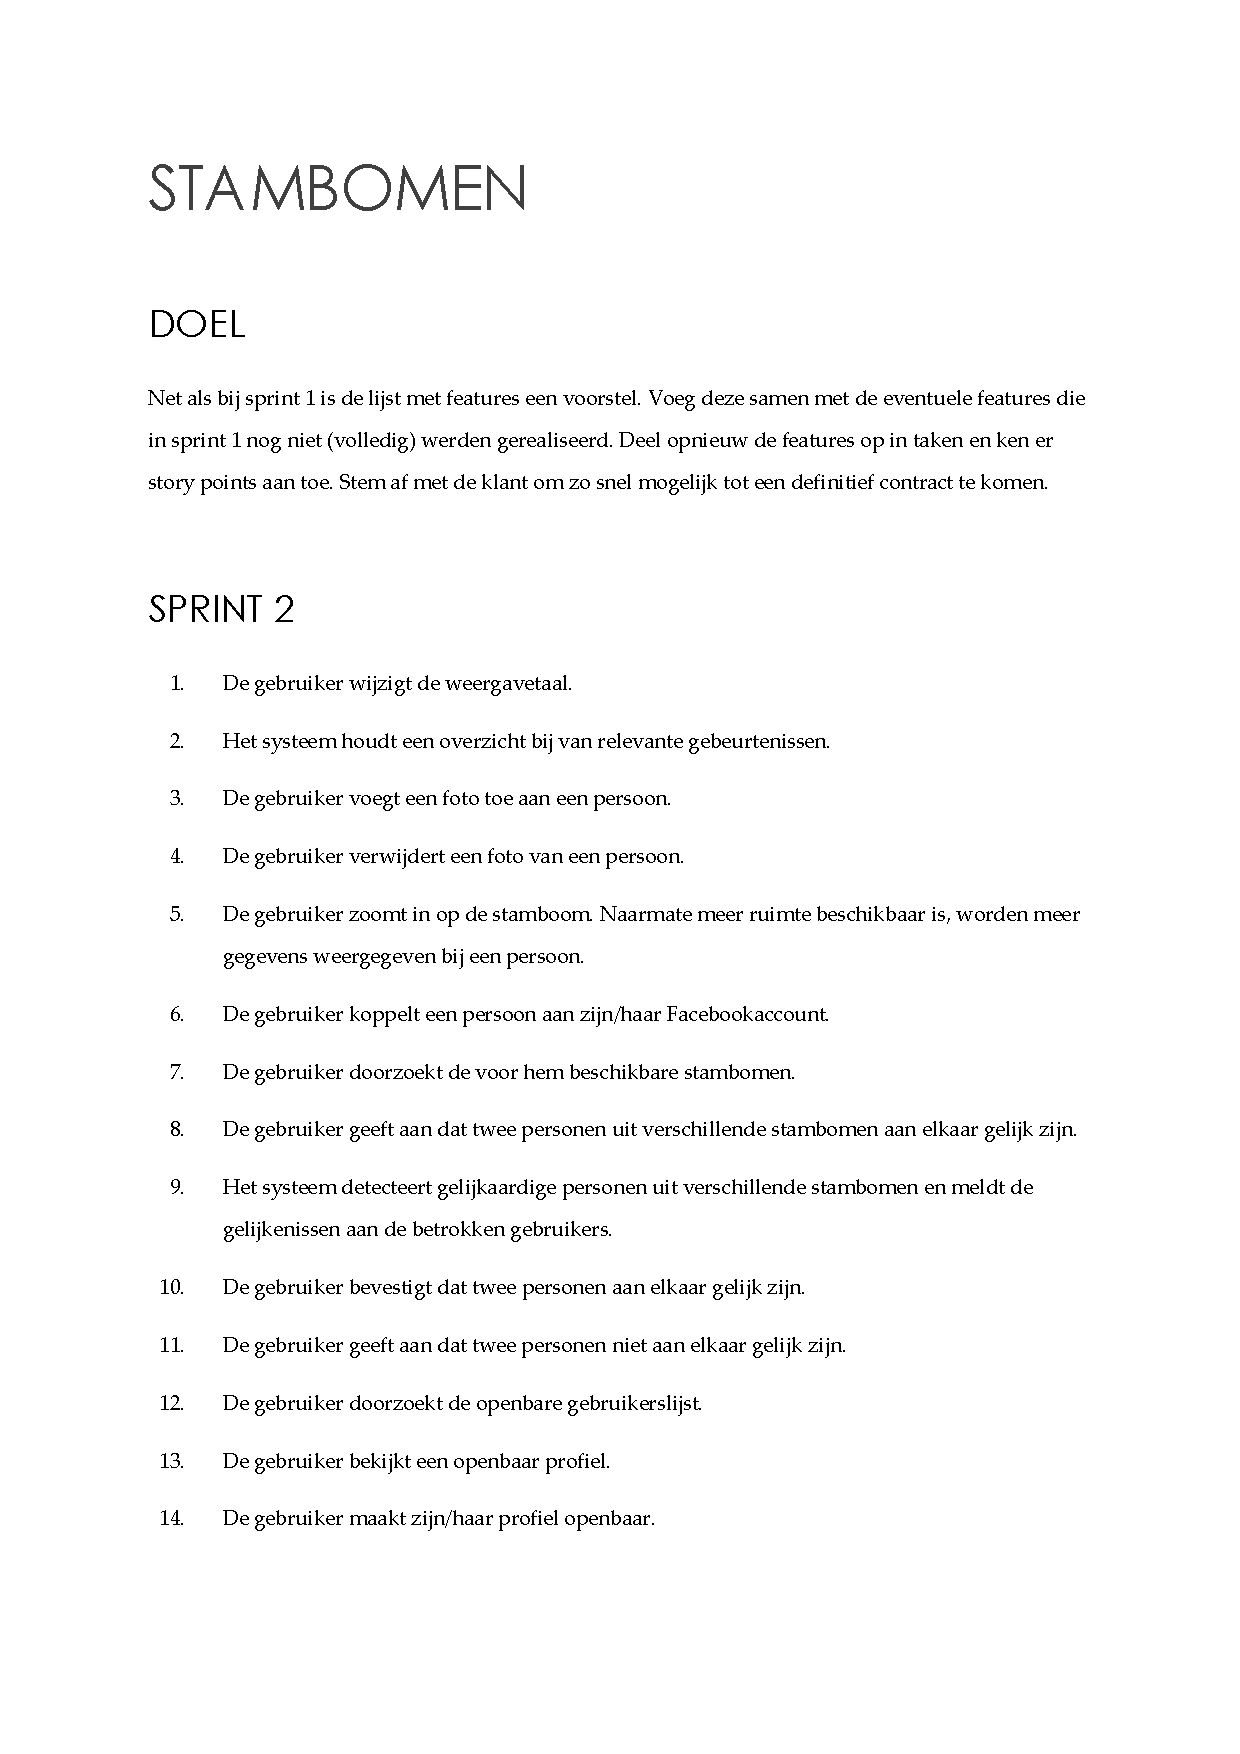
\includepdf[pages=-,pagecommand=\section{Opdracht sprint 2}\label{sec:opdrachtsprint2}, scale=0.80]{Files/stambomen-sprint2.pdf}

\end{document}

